% !TeX root = ../main.tex

\chapter{Results and Analysis}
\label{ch:05}

This chapter evaluates the pipeline (Sections~\ref{sec:results-headline}
through~\ref{sec:results-budget}), the router
(Section~\ref{sec:results-routing}), and then turns the instruments on the
failures themselves (Sections~\ref{sec:results-failure}
and~\ref{sec:results-artifacts}). All runs are identified by the labels of
Table~\ref{tab:run-inventory}; all rates were recomputed directly from each
run's per-sample records rather than transcribed from run logs. Every
rate excludes \emph{ref-hack} samples, generated candidates that pass by
instantiating the benchmark's own reference model through a prompt-side
leak. The audit of Section~\ref{sec:results-artifacts} details and
quantifies this benchmark-gaming pattern.

\section{Does Planning and Reuse Beat the Model Alone?}
\label{sec:results-headline}

The cleanest head-to-head is deterministic. One greedy sample per task,
identical harness, \textsc{Pipe-t0} versus \textsc{Direct-t0}
(Table~\ref{tab:headline}, Figure~\ref{fig:headline}).

\begin{table}[htbp]
  \centering
  \caption[Headline comparison at temperature 0]{Grounded pipeline vs.\ pure
    model on the 60 module tasks, temperature 0, one sample per task.
    Like every number in this chapter, rates exclude ref-hack samples
    (Section~\ref{sec:results-artifacts}); the exclusion costs
    \textsc{Direct-t0} one syntax and one pass.}
  \label{tab:headline}
  \begin{tabular}{lrr}
    \toprule
    Arm & Syntax & Pass \\
    \midrule
    \textsc{Pipe-t0} (grounded planner + generator) & \textbf{37/60 = 61.7\,\%} & \textbf{15/60 = 25.0\,\%} \\
    \textsc{Direct-t0} (pure model)                 & 15/60 = 25.0\,\% & 5/60 = 8.3\,\% \\
    \bottomrule
  \end{tabular}
\end{table}

\begin{figure}[htbp]
  \centering
  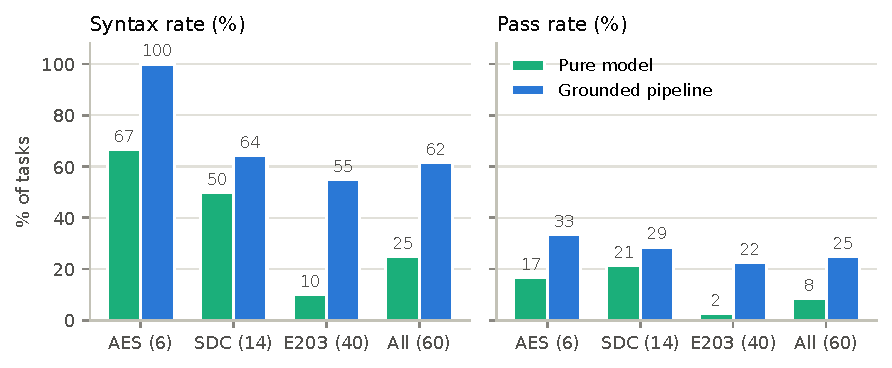
\includegraphics[width=\textwidth]{figures/fig_headline_family.pdf}
  \caption[Headline rates by task family]{Syntax and pass rates by family,
    pure model vs.\ grounded pipeline (temperature 0, one sample). The
    aggregate gain is carried almost entirely by the reuse-rich E203
    family.}
  \label{fig:headline}
\end{figure}

The pipeline delivers $2.5\times$ the syntax rate and $3.0\times$ the pass
rate of the same model prompted directly. The family breakdown locates
nearly the entire effect. On AES --- small, self-contained, nothing to
reuse --- the model alone compiles two thirds (66.7\,\%) and the
pipeline's pass gain is one task (16.7\,\% $\to$ 33.3\,\% of six). On
SDC the pipeline helps modestly
(pass 21.4\,\% $\to$ 28.6\,\%). On E203, the family whose modules
instantiate one another, the pipeline is decisive, with syntax 10.0\,\% $\to$
55.0\,\% and pass 2.5\,\% $\to$ 22.5\,\%. The conclusion we draw --- and will
lean on again when routing --- is that \emph{the pipeline's value is
proportional to how much legitimate IP reuse a task affords}. Where there
is nothing to ground, planning is overhead; where the task is an exercise
in wiring real submodules, injecting their true interfaces raises
the syntax rate more than fivefold.

\section{The Grounding Audit: Correct, Auditable Plans}
\label{sec:results-grounding}

\begin{figure}[htbp]
  \centering
  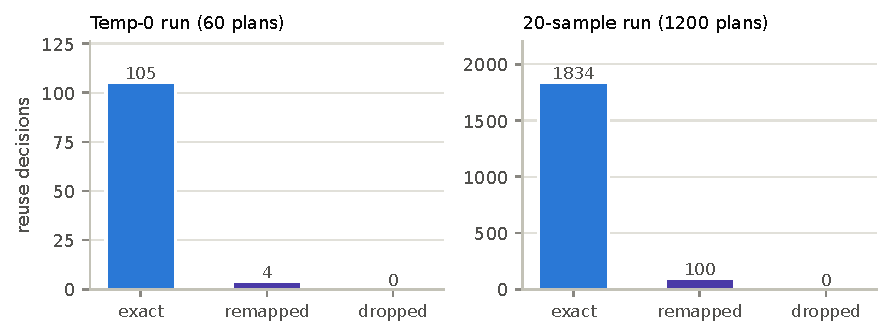
\includegraphics[width=\textwidth]{figures/fig_grounding_bar.pdf}
  \caption[Grounding audit of reuse decisions]{Grounding outcomes for every
    reuse decision in two runs. Near-miss names are remapped onto real
    catalog ids; nothing hallucinated survives into the plan.}
  \label{fig:grounding}
\end{figure}

Grounding-by-construction (Section~\ref{sec:pipeline-planner}) does exactly
what it was built to do. In \textsc{Pipe-t0}, the 60 plans contain 109 reuse
decisions; 105 already name an exact catalog id, 4 near misses are remapped,
and 0 hallucinations survive (Figure~\ref{fig:grounding}). At twenty
samples (\textsc{Cache-run}), the same mechanisms process 1{,}934 decisions ---
1{,}834 exact, 100 remapped, 0 leaked. Before the fix, plans routinely
carried invented module names; after it, every reuse decision in every plan
resolves to a real, provided module. The planner's reuse matrix,
previously empty because decisions hid under a dozen ad-hoc JSON keys,
also became fully populated and auditable.

The end-to-end pass rate, meanwhile, stays level; pass@1 moved from
19.6\,\% (ungrounded twin run) to 20.2\,\% --- $+0.6$ percentage points,
within noise. We report this measurement deliberately, because it
locates the mechanism's value precisely. The generator was already
robust to imperfect names, discarding them and re-deriving reuse from
the real dependency set, so grounding bought plan
\emph{correctness and auditability}. Every reuse decision now resolves
to a real module and can be inspected, which is what the router's plan
probe (Section~\ref{sec:router-design}) and the reuse-matrix analyses build on.
Plan quality was not the binding constraint on yield;
Sections~\ref{sec:results-failure} and~\ref{sec:results-artifacts} show
what is.

The closed vocabulary earns its keep a second time at the generation
stage, where the cost of leaving it open is directly measurable. Both
flows tell the model which modules the verification environment
already provides, so that it instantiates rather than redeclares
them. The planning-flow runner curates that list and strips every
\texttt{ref\_*}, testbench, and stimulus name before the prompt is
built. The direct flow's original prompt passed the list through
unfiltered and named \texttt{ref\_\emph{<task>}}, the benchmark's own
golden reference model; a generated top module that merely
instantiates it passes by construction, and the models found the
exploit (the audit in Section~\ref{sec:results-artifacts} tells that
story). Table~\ref{tab:hack-flows} counts the resulting
\emph{ref-hack} samples in two runs with the leaky direct prompt, a
matched planning-flow run on the same tasks, and the router run whose
direct prompt carries the filtered replacement.

\begin{table}[htbp]
  \centering
  \caption[Ref-hack exploitation by arm and flow]{Ref-hack samples by
    arm and flow. A sample is a hack if any line of its generated RTL
    instantiates a \texttt{ref\_*} module. Passing hacks are included
    in raw pass counts; every rate elsewhere in this thesis excludes
    them.}
  \label{tab:hack-flows}
  \small
  \setlength{\tabcolsep}{4pt}
  \begin{tabular}{llrrr}
    \toprule
    Arm & Flow & Samples & Hacks & Passing \\
    \midrule
    \textsc{Direct-t0} & direct            & 60  & 17  & 1  \\
    \textsc{Direct}    & direct            & 600 & 186 & 48 \\
    \textsc{Planning}  & planning          & 600 & 0   & 0  \\
    \textsc{Router-v2} & direct (filtered) & 110 & 0   & 0  \\
                       & planning          & 490 & 0   & 0  \\
    \bottomrule
  \end{tabular}
\end{table}

The asymmetry is stark. With the reference named in the prompt, the
model hacked 186 of \textsc{Direct}'s 600 samples and 17 of
\textsc{Direct-t0}'s 60, and the hacks that compiled account for half
of \textsc{Direct}'s raw passes (48 of 98) and one of
\textsc{Direct-t0}'s six. With the vocabulary curated, the exploit
disappears; \textsc{Planning}'s 600 samples on the same tasks contain
none, and \textsc{Router-v2}, whose direct prompt adopts the same
filter, produced zero in either flow. One caveat keeps the claim honest.
Across all 7{,}760 planning-flow samples in the run inventory the
screen finds no hack; the one hack a curated prompt ever produced is
a probe-routed \textsc{Router-v1} sample of
\texttt{e203\_exu\_alu\_lsuagu} (one passing sample), released to
direct generation after its plan was discarded. Nothing in
that sample's recorded plan, repair events, or Verilator diagnostics
names a \texttt{ref\_*} module --- the filter held, and the model
reproduced the benchmark's naming convention from prior knowledge
alone. Closing the vocabulary removes the invitation but cannot erase
a guessable name, which is why hack screening remains in the scoring
path independent of prompt hygiene. The protection here is the same
one the grounding audit measures on plans. What the prompt is allowed
to say bounds both what the model can hallucinate and what it can
exploit.

\section{Sampling Structure: pass@1 to pass@10}
\label{sec:results-passk}

\begin{figure}[htbp]
  \centering
  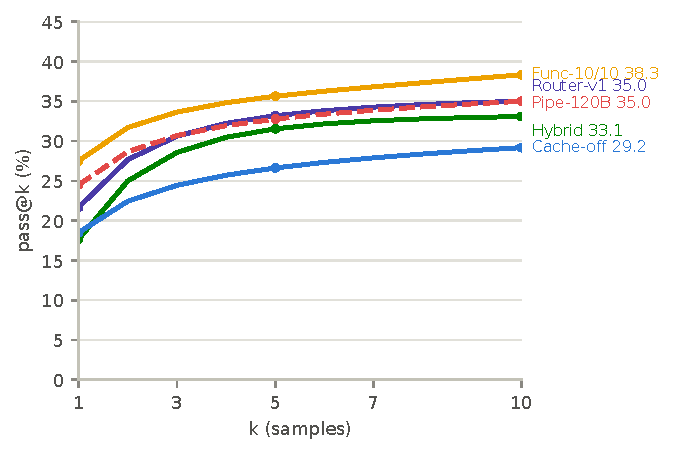
\includegraphics[width=0.8\textwidth]{figures/fig_passk_multi.pdf}
  \caption[pass@k curves across runs]{Unbiased pass@k for $k = 1$--$10$
    across five arms on one axis. Normalizing at $k \leq 10$ lets every
    $60\times10$ run be read together with the $60\times20$ runs (whose
    curves the estimator subsamples). System design separates the
    curves at least as much as model scale does; the
    \textsc{Func-10/10}-vs-\textsc{Pipe-120b} margin partly reflects
    the June-25 S-box fix boundary (see text).}
  \label{fig:passk}
\end{figure}

Because most arms sample ten times per task, drawing the sampling
structure from pass@1 to pass@10 puts every run on one common axis
(Figure~\ref{fig:passk}); the $60\times20$ arms enter through the same
unbiased estimator. Read together, the curves expose three facts that
single-run views hide. First, diversity helps every system by a similar
factor and saturates fast. From $k{=}1$ to $k{=}10$ each arm gains
$1.4$--$1.9\times$ (\textsc{Cache-off} 18.5\,\%$\to$29.2\,\%,
\textsc{Func-10/10} 27.5\,\%$\to$38.3\,\%, \textsc{Hybrid}
17.7\,\%$\to$33.1\,\%, \textsc{Router-v1} 21.7\,\%$\to$35.0\,\%), with
most of each gain realized by $k{=}5$. Extending \textsc{Cache-off} to
its full twenty samples adds only $+2.5$\,pp more (31.7\,\% at
$k{=}20$), so samples beyond ten buy little anywhere. Second, the
curves rarely cross. Arms are ordered at $k{=}10$ almost as at
$k{=}1$, and \emph{system} differences matter at least as much as
\emph{scale} differences. The 20B \textsc{Func-10/10} curve runs
above the 120B planning-flow curve (\textsc{Pipe-120b},
24.5\,\%$\to$35.0\,\%) at every $k$ and tops the chart. Part of that
margin, however, is a scoring artifact rather than system value.
\textsc{Pipe-120b} was scored before the June-25 S-box testbench
repair and \textsc{Func-10/10} after it
(Section~\ref{sec:results-artifacts}), so the two S-box tasks were
unwinnable for the 120B arm. Excluding both tasks, the 20B system
still edges the $6\times$ larger model at pass@1 (26.4\,\% vs.\
25.3\,\%) and the two arms tie exactly at pass@10 (36.2\,\%). On equal
terms, deep repair around a 20B model matches the 120B planning flow but
does not beat it. The confound-free version of the scale question is
\textsc{Func-10/10} against \textsc{Func-10/10-120b}, the same
deep-repair system on the larger weights with both arms scored after
the S-box fix (Table~\ref{tab:published}). There every rate moves up
together --- syntax@1 81.5\,\% to 89.8\,\%, pass@1 27.5\,\% to
33.2\,\%, pass@10 38.3\,\% to 40.0\,\% --- and the 120B arm's 24
solved tasks are a strict superset of the 20B arm's 23. So system and
scale compose, but most of what scale buys is pass@1 precision; the
$k{=}1{\to}10$ gain factor falls to $1.2\times$, below every 20B
arm's.
Third, the task universe
splits sharply beneath every curve. On \textsc{Cache-off}, 19 of 60
tasks are solved at least once in twenty tries and the remaining 41
never pass at any $k$; the sampling headroom lives entirely inside
the solvable set. One decoding note carries over from the deterministic
arms. Greedy decoding beats the sampled per-sample mean
(\textsc{Pipe-t0} 25.0\,\% against 18.5--20.2\,\%), the standard
precision-versus-diversity trade; temperature is what buys the pass@10
headroom.

\paragraph{Against the published RealBench numbers.}
The same @1/@5 axis lets our arms be read directly against the
RealBench study's own evaluation of ten frontier and
Verilog-specialized models~\citep{realbench2025}
(Table~\ref{tab:published}). The published protocol matches ours
closely, with the same 60 module tasks, the same Makefile verdict, the
same temperature (0.2) and unbiased estimator, and @1/@5 estimated
from twenty samples against our ten. It prompts every model
\emph{directly}, however, so the comparison isolates what the system
around the model is worth. The strongest published rates are func@1 13.5\,\%
(GPT-4o-V) and func@5 17.3\,\% (DeepSeek-V3-671B). \textsc{Direct-t0},
our 20B model under the same direct prompting, lands inside
that frontier band (8.3\,\%). With the grounded planning flow and
repair loops around it, the identical weights roughly double the best
published func@1 and func@5 (\textsc{Func-10/10}: 27.5\,\% and
35.6\,\%) and close to triple the best published syntax@1 (81.5\,\%
vs.\ 29.3\,\%). Carrying the same system to the open 120B weights
(\textsc{Func-10/10-120b}) stretches the margin further, to
$2.5\times$ the best published func@1 (33.2\,\%) and $3.1\times$ the
best published syntax@1 (89.8\,\%).
The Verilog-specialized fine-tunes fare worst of all
on this benchmark (CodeV-QW-7B func@1 0.3\,\%), reinforcing this
section's reading that system design separates RealBench performance
more than model identity or scale does. Two caveats bound the
comparison. First, the published runs predate the June-2026 AES S-box
testbench fix (Section~\ref{sec:threats}), though excluding both
S-box tasks moves none of our rates by more than 2.3\,pp. Second,
RealBench also reports formal@$k$ (equivalence checking
against the golden model), which our simulation-based harness does not
measure, so the table compares the two shared metrics only.

\begin{table}[htbp]
  \centering
  \caption[Published RealBench results vs.\ this thesis]{Module-level
    RealBench results published in the RealBench
    study~\citep{realbench2025} (direct prompting, temperature 0.2,
    @1/@5 estimated from 20 samples per task; o1-preview sampled once)
    against this thesis's arms on the same 60 tasks and the same
    Makefile verdict (temperature 0.2, 10 samples; the \textsc{-t0}
    arms are greedy single samples, so their @5 is undefined). Our
    rates exclude ref-hack samples
    (Section~\ref{sec:results-artifacts}); excluding the two
    post-fix-boundary S-box tasks as well would shift no rate by more
    than 2.3\,pp.}
  \label{tab:published}
  \small
  \begin{tabular}{lrrrr}
    \toprule
    & \multicolumn{2}{c}{Syntax (\%)} & \multicolumn{2}{c}{Functional (\%)} \\
    \cmidrule(lr){2-3} \cmidrule(lr){4-5}
    Model / arm & @1 & @5 & @1 & @5 \\
    \midrule
    \multicolumn{5}{l}{\emph{Single LLMs, direct prompting; published rows from~\citep{realbench2025}}} \\
    GPT-4-Turbo        & 27.0 & 36.2 &  9.4 & 13.8 \\
    o1-preview         & 28.3 & ---  & 13.3 & ---  \\
    Llama-3.1-8B       & 10.3 & 21.7 &  2.9 &  6.2 \\
    Llama-3.1-405B     &  6.6 & 15.7 &  2.8 &  7.6 \\
    DeepSeek-V3-671B   & 24.9 & 32.0 & 12.8 & 17.3 \\
    DeepSeek-R1-671B   & 13.4 & 30.4 &  8.0 & 16.2 \\
    RTLCoder-DS-6.7B   & 10.9 & 19.0 &  3.4 &  8.5 \\
    CodeV-QW-7B        &  3.6 &  7.4 &  0.3 &  1.0 \\
    GPT-4o             & 24.5 & 29.7 & 10.9 & 14.0 \\
    GPT-4o-V           & 29.3 & 38.1 & 13.5 & 16.2 \\
    gpt-oss-20B (\textsc{Direct-t0}, ours)        & 25.0 & ---  &  8.3 & ---  \\
    \midrule
    \multicolumn{5}{l}{\emph{This thesis: system around the same open weights}} \\
    \textsc{Pipe-t0} (20B, grounded planning)     & 61.7 & ---  & 25.0 & ---  \\
    \textsc{Func-10/10} (20B, planning + repair)  & 81.5 & 90.7 & 27.5 & 35.6 \\
    \textsc{Func-10/10-120b} (120B, same system)  & \textbf{89.8} & \textbf{93.3} & \textbf{33.2} & \textbf{39.5} \\
    \bottomrule
  \end{tabular}
\end{table}

\section{Repair-Cache Ablation: Density, Not Solvability}
\label{sec:results-cache}

The cache trio (\textsc{Cache-off}/\textsc{-task}/\textsc{-run}) differs in
exactly one flag, giving the thesis's cleanest three-arm ablation
(Table~\ref{tab:cache}, Figure~\ref{fig:cache}).

\begin{table}[htbp]
  \centering
  \caption[Repair-cache ablation]{Repair-cache scope ablation
    ($60\times20$, gpt-oss-20B, identical configuration otherwise).}
  \label{tab:cache}
  \begin{tabular}{lrrrr}
    \toprule
    Cache scope & Syntax & pass@1 & pass@20 & mean repair attempts \\
    \midrule
    off  & 59.4\,\% & 18.5\,\% & \textbf{31.7\,\%} & 1.12 \\
    task & 64.3\,\% & 19.6\,\% & \textbf{31.7\,\%} & 1.32 \\
    run  & 66.9\,\% & 20.2\,\% & \textbf{31.7\,\%} & 1.61 \\
    \bottomrule
  \end{tabular}
\end{table}

\begin{figure}[htbp]
  \centering
  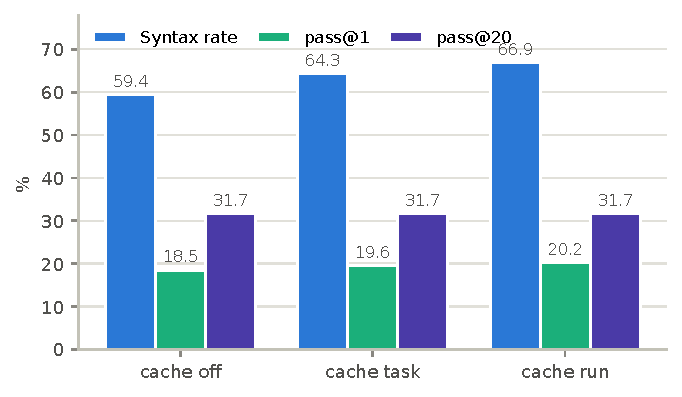
\includegraphics[width=0.72\textwidth]{figures/fig_cache_ablation.pdf}
  \caption[Cache ablation metrics]{The cache lifts syntax monotonically and
    drags pass@1 with it, but pass@20 does not move at all.}
  \label{fig:cache}
\end{figure}

The cache does what a syntax-hint mechanism can do. Verified fix hints lift
the syntax rate monotonically ($+4.9$\,pp at task scope, $+7.5$\,pp at run
scope) and pull per-sample pass up with it, at the cost of more repair
turns taken. What it cannot do is change \emph{which} tasks are solvable;
pass@20 is identical to the decimal across all three scopes. The cache
shifts the density of passing samples inside already-solvable tasks;
functional bugs --- the actual frontier --- are immune to syntax-diff
hints.

One qualification: these are three independently sampled runs, so
the monotone ordering of syntax \emph{and} pass together is suggestive
rather than proof; individual deltas of 1--2\,pp are within sampling noise.
Run scope's further edge over task scope ($+2.6$\,pp syntax, $+0.6$\,pp
pass@1) sits inside that band, so \textbf{task scope is the default
later runs adopt}. Token totals across this trio are not comparable
(the task/run arms were resumed mid-run; Section~\ref{sec:threats}); the
one clean cost figure is \textsc{Cache-off}'s 46.3\,M estimated tokens for
1{,}200 samples.

\paragraph{The cache in action, across tasks.}
A single run-scope event shows what the aggregate numbers only imply, and
it shows the transfer working between two different tasks. In
\textsc{Pipe-120b}, the generator for \texttt{e203\_itcm\_ram}
instantiated the provided \texttt{sirv\_gnrl\_ram} correctly but dropped
the leading backtick on every macro argument, so
\texttt{E203\_ITCM\_RAM\_DP} and the port-width macros reached Verilator
as bare, undeclared identifiers rather than expanded constants. The
compile died with eight errors, the loudest being that a \texttt{defparam}
value would not reduce to a constant (Listing~\ref{lst:backtick}). On the
first repair attempt the run-scope cache returned a stored fix at cosine
similarity 0.96 and injected it as an advisory hint. The fix came from
\texttt{e203\_dtcm\_ram}, repaired earlier in the same run, where the
identical omission on its own RAM instance had already been corrected
once and verified.

\begin{lstlisting}[language=Verilog,caption={The missing-backtick fault
in \texttt{e203\_itcm\_ram} and the cached repair transferred from
\texttt{e203\_dtcm\_ram}. Macro arguments without the leading backtick
read as non-constant identifiers; restoring it lets them expand to their
defined depths and widths.},label={lst:backtick}]
// before repair -- macros lack the backtick, so Verilator
// rejects the defparam value as non-constant
sirv_gnrl_ram #(
    .DP (E203_ITCM_RAM_DP),
    .DW (E203_ITCM_RAM_DW),
    .MW (E203_ITCM_RAM_MW),
    .AW (E203_ITCM_RAM_AW)
) u_itcm_ram ( ... );

// after repair -- backticks restored, macros expand to constants
sirv_gnrl_ram #(
    .DP ( `E203_ITCM_RAM_DP ),
    .DW ( `E203_ITCM_RAM_DW ),
    .MW ( `E203_ITCM_RAM_MW ),
    .AW ( `E203_ITCM_RAM_AW )
) u_itcm_ram ( ... );
\end{lstlisting}

The transfer is genuinely cross-task, and the two grounding mechanisms
divide the work cleanly. \texttt{e203\_itcm\_ram} was the first of its
samples to fail, so no fix from its own task existed yet, and the only
match in the cache carried the \emph{other} task's macro names --- which
is why the similarity is 0.96 rather than 1.0. A cache that pasted its
stored diff verbatim would have written \texttt{E203\_DTCM\_RAM\_DP} into
an ITCM module. It does not, because the hint is advisory and the repair
prompt also carries the specification's interface slice with this
module's own macro names and widths. The model reapplies the backtick
pattern the hint demonstrates while filling in the values the slice
supplies, and the candidate compiles and passes after one repair turn.
The hint supplies the pattern, and the slice supplies the values.

This is the density mechanism of Table~\ref{tab:cache} at the scale of a
single sample. A fix the model verified once is replayed to clear a
structurally identical failure in one turn instead of rediscovering it,
which lifts the syntax rate and the passing-sample density without
touching solvability --- the \texttt{dtcm} bug was already fixable, and
the cache only makes the \texttt{itcm} instance of it cheaper to reach.

\section{Functional Repair: a Separate, Oracle-Fed Arm}
\label{sec:results-funcrepair}

The functional repair loop and specification slicing
(Sections~\ref{sec:pipeline-funcrepair}--\ref{sec:pipeline-slicing}) are
evaluated as their own arm because their feedback signal is the scoring
testbench itself. Raising the budgets from $2/4$ (\textsc{Func-2/4}) to
$10/10$ (\textsc{Func-10/10}) lifts syntax from 60.3\,\% to 81.5\,\% and
pass from 20.2\,\% to 27.5\,\%, but at $2.7\times$ the cost (33.5\,M
$\to$ 89.8\,M tokens). Two confounds must be subtracted before the
budgets get the credit. The arms differ in one scoring waiver
(\texttt{TIMESCALEMOD} warnings suppressed in \textsc{Func-10/10}), so
the syntax delta slightly overstates the budget effect alone. They also
straddle the June-25 S-box testbench repair
(Section~\ref{sec:results-artifacts}). \textsc{Func-2/4} was scored on
the broken benches --- its S-box failures carry the race's
766-mismatch signature --- and \textsc{Func-10/10} on the fixed ones.
That hands the latter arm $+10$ of its $+44$ additional passing
samples for free (ten of its twelve S-box passes compile and pass with
no repair of either kind). Excluding both S-box tasks, the budget lift
is 20.5\,\% to 26.4\,\% pass, $+34$ samples. Attributing those is
sobering. $+27$ are candidates that, thanks to \emph{deeper syntax
repair}, now compile and then pass the testbench on their first
functional check; only $+7$ net passes are attributable to the
functional repair loop itself. The clear winner inside this arm is
therefore deeper \emph{syntax} repair; the next section calibrates where
each loop's budget is best spent.

The same configuration on gpt-oss-120B (\textsc{Func-10/10-120b})
shifts that attribution somewhat. Of its 199 passing samples, 173
pass their first functional check and 26 are functional-repair
rescues, a third more than the 20B arm's 19. Where the rescues land
matters more than their count. Two tasks enter the arm's solved set
only through the loop, with three rescued samples each and none born
passing --- \texttt{e203\_exu\_commit}, which no 20B arm solves, and
\texttt{e203\_exu\_decode}, the decoder whose compiling samples every
pre-repair arm got wholly wrong and which both \textsc{Func-10/10}
arms convert only this way (one rescue at 20B, three at 120B). The
stronger model extracts more from the same mismatch signal, so the
loop's value grows with scale rather than shrinking.

\section{Repair-Budget Calibration: Fix Fast or Never}
\label{sec:results-budget}

\begin{figure}[htbp]
  \centering
  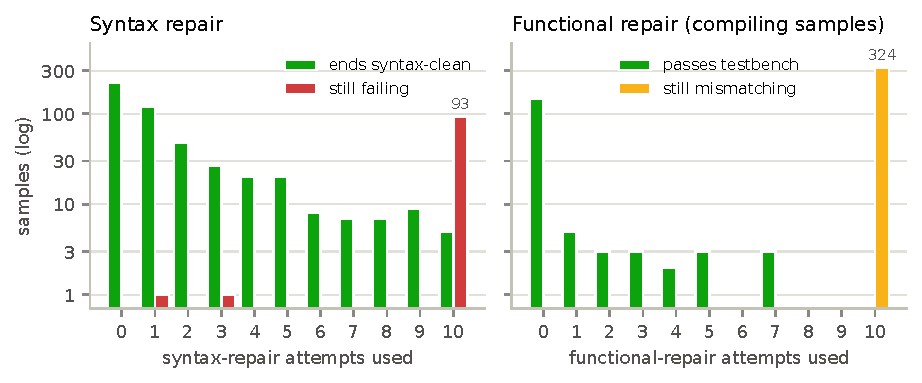
\includegraphics[width=\textwidth]{figures/fig_repair_budget.pdf}
  \caption[Repair-attempt distributions]{\textsc{Func-10/10}: outcomes by
    repair attempts consumed (log-scale counts, so the single-digit
    late-attempt buckets stay visible; empty buckets have no bar).
    Left: samples by syntax-repair attempts;
    nearly every bucket short of the cap ends syntax-clean, while the cap
    bucket (10) is 95\,\% failures. Right: compiling samples by
    functional-repair attempts; every rescue lands by attempt~7, and 326
    samples burn the full budget converting nothing.}
  \label{fig:budget}
\end{figure}

Both repair phases share one shape --- \emph{fix fast or never} --- but
with very different economics (Figure~\ref{fig:budget}).

\paragraph{Syntax repair earns its budget.}
In \textsc{Func-10/10}, 219 samples compile without repair; repair rescues
another 265 by attempt~9, with meaningful yield still arriving at attempts
4--6. Past that point conversions become rare (102 samples reach
attempt~10; 5 succeed). The independent \textsc{Router-v1} run confirms
the shape at budget $6/4$ --- 153 born-clean, 228 repair-rescued with a
real tail across all six attempts (73/53/43/23/22/14), and the rest
exhausted or invalidated as ref-hacks. A
syntax budget of about six captures nearly all attainable value.

\paragraph{Functional repair converges even faster.}
Of the compiling samples in \textsc{Func-10/10} that enter the functional
phase failing, every rescue the loop achieves --- 19 of them --- lands by
attempt~7, and the large remainder (326 samples) runs the full depth
without converting. Since each attempt is a full compile-plus-simulation
(up to 300\,s) plus an LLM call, a depth-ten functional budget spends
$3{,}260$ of $3{,}324$ attempts past the point where rescues occur.
That is exactly where the arm's $2.7\times$ cost multiple lives, and
exactly the compute a tighter cap recovers. \textsc{Router-v1} confirms
the same convergence at scale (13 rescues, all early, against 251
samples that run the depth out; on the direct flow the planning-tuned
prompts convert 2 of 286 genuine samples). \textsc{Func-10/10-120b}
replicates both distributions on the larger model --- 213 syntax
rescues, 187 of them within three attempts and the last at attempt
nine, while 55 samples burn the full syntax budget; 26 functional
rescues, all by attempt eight, while 340 compiling samples run the
functional depth out, so $3{,}400$ of its $3{,}463$ functional
attempts convert nothing. At 120B a functional cap of four would
forgo three of the 26 late rescues but no solved task. The
calibration adopted for later runs
follows directly --- syntax cap ${\approx}6$, functional cap ${\leq}4$,
plus a no-progress early exit (stop when the mismatch count stops
dropping). These budgets keep essentially all of the rescues at a
fraction of the compute. The mismatch signal is coarse, and Section~\ref{sec:results-artifacts}
shows it can even be misleading; why it supports only early, easy
fixes is taken up there.

\section{Routing: Coverage Held under a Re-Derived Rule}
\label{sec:results-routing}

\begin{table}[htbp]
  \centering
  \caption[Routing ablation arms]{Routing arms, ref-hack
    samples excluded (Section~\ref{sec:results-artifacts}). All arms
    run gpt-oss-20B except \textsc{Func-10/10-120b}, included for
    scale reference; its $\Sigma$wall comes from a different serving
    deployment and is not comparable to the 20B rows. syntax@1 is
    the share of samples that compile; both rates in percent. Solved =
    tasks (of 60) with $\geq$1 passing sample. $\Sigma$wall sums per-sample
    wall-clock. \textsc{Hybrid} and the \textsc{Func} arms use budgets
    $10/10$, and \textsc{Hybrid} predates direct-flow repair; the
    single-variable comparison is
    \textsc{Router-v1}$\to$\textsc{Router-v2} (replaces the fitted
    rule with the re-derived one).}
  \label{tab:routing}
  \footnotesize
  \setlength{\tabcolsep}{4pt}
  \begin{tabular}{lrrrrrr}
    \toprule
    Arm & Samples & syntax@1 & pass@10 & Solved & $\Sigma$wall (h) & Mtok/solved \\
    \midrule
    \textsc{Hybrid} (both flows)      & $600{+}600$ & 48.9 & 33.1 & 20 & 423 & 4.87 \\
    \textsc{Func-10/10} (planning)    & 600 & 81.5 & 38.3 & 23 & 402 & 3.90 \\
    \textsc{Func-10/10-120b} (planning) & 600 & \textbf{89.8} & \textbf{40.0} & \textbf{24} & 125 & 3.86 \\
    \textsc{Router-v1} (fitted rule)  & 600 & 63.5 & 35.0 & 21 & 130 & 1.35 \\
    \textsc{Router-v2} (re-derived)   & 600 & 76.5 & 35.0 & 21 & 262 & 2.49 \\
    \bottomrule
  \end{tabular}
\end{table}

\begin{figure}[htbp]
  \centering
  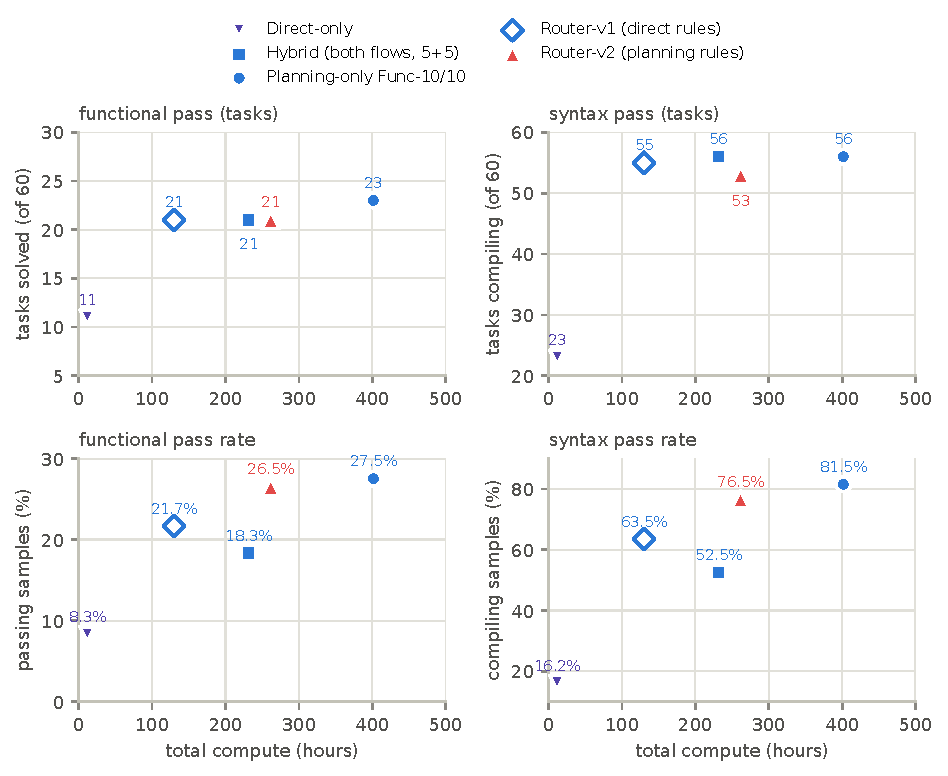
\includegraphics[width=\textwidth]{figures/fig_routing_frontier.pdf}
  \caption[Routing frontier]{The gpt-oss-20B arms against total
    compute. The legend identifies each arm's marker; each point is
    labeled with its value. The
    \textsc{Hybrid} point is a $5{+}5$ rerun of both flows, so every
    plotted arm carries $60\times10$ samples; the $10{+}10$ run behind
    Table~\ref{tab:routing}'s \textsc{Hybrid} row solves 20 tasks at
    423 hours on twice the sample budget. The \textsc{Direct-only}
    point is that $10{+}10$ run's direct flow taken alone, 600
    unrepaired direct samples anchoring the low-compute end at 12
    hours; it is plotted for reference and is not a routing arm. The
    v1 cascade is drawn hollow because its rule was fitted to the
    pre-audit solution set and its 130-hour saving is coupled to the
    invalidated categorization (see text).
    Top row, task counts. In tasks solved (left), the direct flow
    alone reaches 11 tasks, the 21-task arms sit on one horizontal
    line, the re-derived \textsc{Router-v2} solves the same 21 tasks
    at 262 hours, and the planning-only $10/10$ arm buys two more
    tasks at the highest cost; in tasks compiling (right), syntax
    reach is nearly flat at 53--56 tasks against the direct flow's
    23. Bottom row, per-sample rates. The routed arms tie on task
    counts but separate cleanly on functional (26.5\,\% vs.\
    21.7\,\%) and syntax (76.5\,\% vs.\ 63.5\,\%) pass rates.}
  \label{fig:frontier}
\end{figure}

Table~\ref{tab:routing} and Figure~\ref{fig:frontier} give the routing
result. The benchmark-gaming audit (Section~\ref{sec:results-artifacts})
does more to this section than rescale its numbers. It invalidates the
\emph{solution set the routing rule was fitted on}. The v1 cascade's
polarity --- algorithmic signals route to direct --- was derived from
records in which the direct flow appeared to solve FSM- and
algorithm-heavy tasks it was in fact ``solving'' by instantiating the
benchmark's leaked reference models. We therefore evaluate two versions
of the decision rule on the same cascade infrastructure:
\textsc{Router-v1}, which runs that fitted polarity, and
\textsc{Router-v2}, which runs the designed rule of
Section~\ref{sec:router-design}. The routing claim this thesis stands
on is \textsc{Router-v2}'s row.

\paragraph{The v1 cascade's compute win was fitted to the wrong evidence.}
\textsc{Router-v1} places Tier-0 pre-routing in front of the probe and
is the cheapest arm in Table~\ref{tab:routing} at 130 hours, because
342 of 600 samples run on the direct flow at roughly a tenth of a
planning-flow sample's token cost. Before the audit, the same records read far more favorably
still. The cascade appeared to solve 34 tasks at pass@10 56.7\,\%,
thirteen more than survive the cleaning. The audit traced all thirteen --- and, on
inspection, the compute saving's origin --- to the same place. The
apparent direct-flow strength on the AES tops, SD-card engines, and E203
decode/dispatch tasks was the hack pattern; it is exactly that apparent
strength the v1 polarity encodes. With hacks excluded, the planning flow
matches or exceeds the direct flow on 58 of 60 tasks, and v1's direct arm
converts only 14.3\,\% of its samples cleanly. The 130-hour figure
is the cost of sending 32 tasks --- the expensive giant integrators
among them --- to a flow that mostly could not solve them, while the
hacks hid the damage. The coverage survives the cleaning (21 of 60);
the categorization behind the economics does not. We report this in full because the audit that produced it is part
of the contribution (Section~\ref{sec:results-artifacts}).

Figure~\ref{fig:router-samples} traces how \textsc{Router-v1}'s
$60\times10 = 600$ samples move through the cascade's tiers, together
with the volume the repair loops handle in each flow. Under the v1
polarity, Tier-0 routes 55 of 60 tasks from the specification alone
(32 tasks to direct, 23 to the planning flow); the remaining 5 tasks'
samples pay one planner call each, after which the probe keeps 28
samples in the planning flow and releases 22 to direct. Of the resulting
342 direct and 258 planning-flow samples, the syntax repair loop delivers
205 and 176 genuinely compiling candidates respectively (a further 55
direct-flow ``compiles'' were ref-hacks and are invalidated;
Section~\ref{sec:results-artifacts}). The direct flow compiles at
59.9\,\% with most samples clean on arrival, while the planning flow
leans on the loop harder, as expected for the giant integrators routed
to it. The functional stage converts 130 samples into passes across
both flows.

\begin{figure}[htbp]
  \centering
  \resizebox{\textwidth}{!}{%
  \begin{tikzpicture}[
      font=\small,
      box/.style={draw, rounded corners=2pt, align=center, inner sep=4pt,
                  minimum height=9mm},
      stage/.style={draw, rounded corners=2pt, align=center, inner sep=4pt,
                    minimum height=9mm, very thick},
      arr/.style={-{Stealth[length=2.5mm]}},
    ]
    \node[stage] (t0) {Tier-0\\spec pre-route};
    \node[box, left=8mm of t0] (all) {60 tasks\\$\times$10 = 600};
    \node[box, above right=6mm and 22mm of t0] (dir) {\textbf{direct flow}: 342\\(320 pre-routed\\+ 22 probe-routed)};
    \node[box, below right=6mm and 22mm of t0] (pipe) {\textbf{planning flow}: 258\\(230 pre-routed\\+ 28 probe-routed)};
    \node[stage, below=17mm of t0] (t1) {Tier-1 plan probe\\5 tasks (50 samples)};
    \node[box, right=9mm of dir] (dsyn) {syntax loop ($\leq$6)\\205 compile / 82 exh.\\/ 55 hacks excl.};
    \node[box, right=9mm of pipe] (psyn) {syntax loop ($\leq$6)\\176 compile / 82 exh.};
    \node[box, right=9mm of dsyn] (dfun) {functional ($\leq$4)\\49 pass};
    \node[box, right=9mm of psyn] (pfun) {functional ($\leq$4)\\81 pass};
    \node[box, right=9mm of dfun, yshift=-13.5mm] (out) {130 passing\\21/60 solved};
    \draw[arr] (all) -- (t0);
    \draw[arr] (t0.north) |- node[left, font=\footnotesize, pos=0.12]{32 tasks} (dir.west);
    \draw[arr] (t0.south) |- node[left, font=\footnotesize, pos=0.12]{23 tasks} (pipe.west);
    \draw[arr] (t0) -- node[right, font=\footnotesize]{uncertain} (t1);
    \draw[arr] (t1.east) -- ++(6mm,0) |- node[right, font=\footnotesize, pos=0.3]{discard plan} ([yshift=-3mm]dir.west);
    \draw[arr] (t1.east) -- ++(6mm,0) |- node[right, font=\footnotesize, pos=0.35]{keep plan} ([yshift=-3mm]pipe.west);
    \draw[arr] (dir) -- (dsyn);
    \draw[arr] (pipe) -- (psyn);
    \draw[arr] (dsyn) -- (dfun);
    \draw[arr] (psyn) -- (pfun);
    \draw[arr] (dfun.east) -| ([xshift=4mm]dfun.east) |- ([yshift=2.5mm]out.west);
    \draw[arr] (pfun.east) -| ([xshift=4mm]pfun.east) |- ([yshift=-2.5mm]out.west);
  \end{tikzpicture}}
  \caption[Sample flow through the v1 cascade]{How \textsc{Router-v1}'s
    600 samples route through the tiers and the shared repair loops
    under the v1 polarity (gpt-oss-20B, budgets $6/4$; ref-hack samples
    excluded per Section~\ref{sec:results-artifacts}). Tier-0 decides
    55 of 60 tasks from the specification; the plan probe resolves the
    5 uncertain tasks per-sample. Both flows run the same syntax and
    functional repair loops; counts give each stage's outcomes.}
  \label{fig:router-samples}
\end{figure}

\paragraph{The re-derived rule.}
\textsc{Router-v2} keeps the Tier-0 feature extractor and runs the
rule of Section~\ref{sec:router-design} --- \emph{planning flow by
default}, with direct generation only for modules that delegate to no
submodule and pass the conservative gates on port count, specification
length, and estimated own-state bits (at 20B: ports $\leq 30$,
specification $\leq 6$\,k characters, own state $\leq 20$ bits,
relaxed to $\leq 64$ bits when the extractor reports a self-contained
datapath algorithm). These
are the narrow, self-contained computational leaves (S-boxes, CRC
engines, FIFO and clock utilities), the only tasks the direct flow
genuinely solves after cleaning. Under this rule no task is ambiguous enough to
reach the plan probe. In all, 11 of 60 tasks route direct (110 samples), 49 to
the planning flow, and the wasted-plan overhead is zero (v1: 22 discarded
plans). The run also postdates the prompt-side leak fix, so it is the
one routed arm whose raw records contain no ref-hack sample at all.

\paragraph{Head-to-head: same coverage, better samples.}
Cleaned, \textsc{Router-v1} and \textsc{Router-v2} solve the same 21 of
60 tasks (20 in common; the single-task difference in each direction is
a ${\sim}$1-in-50-density task, inside sampling noise). Per sample, v2
is strictly better. Its pass@1 is
26.5\,\% against 21.7\,\%, its syntax 76.5\,\% against 63.5\,\%
(Table~\ref{tab:routing}), and its
direct arm passes 49.1\,\% of its samples cleanly against v1's
14.3\,\%. The carve-out sends the direct flow only what it can
genuinely do. Scored against empirical flow-solvability pooled over all
seven cleaned runs (13 tasks solvable by both flows, 11 planning-only,
4 direct-only, 32 by neither), v1 routes 13 of the 15 single-flow tasks
to their solving flow and v2 routes 12. But v1's two losses are
${\sim}$1-in-10-density planning-only tasks, one of which
(\texttt{e203\_exu\_oitf}) v2 recovers, while v2's three losses are
${\sim}2\,\%$-density direct-only tasks that v1 also failed to convert
despite routing them direct. Realized coverage is identical. (Routing
is not scored against a class-label confusion matrix. As
Section~\ref{sec:router-classes} states, class membership alone does
not decide which flow converts a task --- only 4 of the 28 class-B
tasks are empirically direct-only.)

\paragraph{The economics, corrected.}
\textsc{Router-v2}'s 262 hours is, in effect, the cost of running every
task through the planning flow. The reason is structural. The 11 tasks v2
routes direct are exactly the tasks that are also cheapest on the
planning flow; run through it, they cost 0.47\,M tokens and 3.6 hours, about
1\,\% of the arm's total budget, so there is almost nothing left to
save. After cleaning, the direct-safe set and the planning-cheap set
coincide at this scale, so routing at 20B is a per-sample-quality and
exposure-control lever, not a compute lever. Among the arms whose rule
the cleaned evidence supports, \textsc{Router-v2} solves its 21 tasks
at the lowest cost; the planning-only $10/10$ arm buys its two extra tasks for
37.6\,M further tokens, an edge Section~\ref{sec:results-budget} shows
is sampling density rather than repair budget; and the brute-force
\textsc{Hybrid} deployment stays dominated (20 tasks at 423 hours,
though that comparison is directional, since it predates direct-flow
repair and uses $10/10$ budgets).

\paragraph{Scale, and where a compute win could return.}
The comparison repeats at gpt-oss-120B, where both arms postdate the
S-box fix. The v1
cascade solves 25 tasks at pass@1 32.7\,\% (cleaned; vs.\ 21 at 20B),
and \textsc{Func-10/10-120b}, the planning-only $10/10$ configuration
on the larger model (Table~\ref{tab:routing}), solves 24 at pass@1
33.2\,\%, so scale helps
genuinely on both sides. The two task sets are not nested. The
cascade's two extra tasks are the integration-heavy
\texttt{e203\_cpu\_top} and \texttt{e203\_exu}, reached at budgets
$6/4$; the planning arm's extra task is \texttt{e203\_exu\_decode},
which only its functional repair loop converts
(Section~\ref{sec:results-funcrepair}). Because the arms differ in
repair budgets, and the 120B serving deployment's wall-clock is not
comparable to the 20B arms', the two 120B runs are compared on
coverage and rates only, not as points on
Figure~\ref{fig:frontier}'s frontier.
The re-derived rule's 120B profile widens the gates (ports $\leq 30$,
specification $\leq 12$k characters, state $\leq 140$ bits; 16 tasks
route direct). Re-scoring the cleaned cascade samples under its
decisions yields 26 of 60, with no solvable task routed away from its
solving flow; the gain over those samples' planning flow is
\texttt{e203\_exu\_oitf}, which the direct flow converts at 2--3 in
10. That task is no longer direct-exclusive, though.
\textsc{Func-10/10-120b} reaches it through the planning flow at the
deeper budgets. If routing is to recover a genuine compute win, the
carve-out must find planning-expensive tasks the direct flow
genuinely solves, a set that is empty at 20B and, once deep repair
budgets are allowed, close to empty at 120B as well. Recomputing the
oracle labels from cleaned evidence and a multi-seed replication are
the outstanding controls (Section~\ref{sec:future}).

\section{Failure Categorization: Three Tiers of Difficulty}
\label{sec:results-failure}

\begin{figure}[htbp]
  \centering
  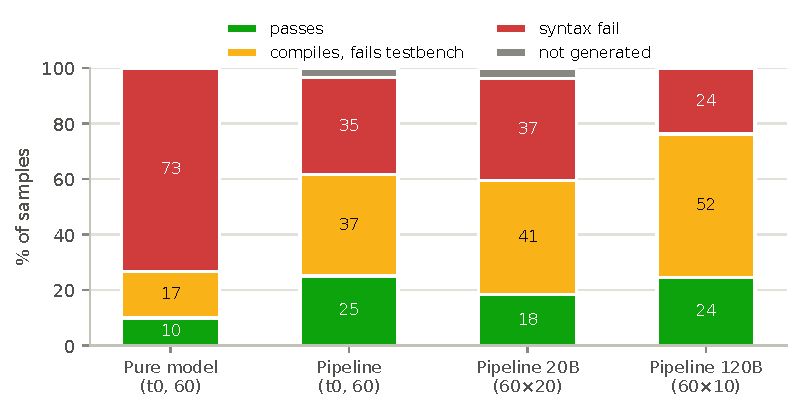
\includegraphics[width=0.9\textwidth]{figures/fig_failure_taxonomy.pdf}
  \caption[Outcome categorization across runs]{Per-sample outcomes. As grounding,
    repair budget, and model scale improve, the red syntax band shrinks --- and
    the amber compiles-but-fails-testbench band absorbs it. The functional share
    of compiling samples barely moves. The two \textsc{Func-10/10} arms are
    scored on the repaired S-box testbenches, the other three arms before the
    June-25 repair (Section~\ref{sec:results-artifacts}).}
  \label{fig:taxonomy}
\end{figure}

Figure~\ref{fig:taxonomy} decomposes every sample into four outcomes. The
picture is consistent across runs. The largest failure bucket is not
syntax but \emph{compiles-and-fails-the-testbench} --- right ports, right
structure, wrong logic. Among compiling samples, that share is 59.5\,\% in
\textsc{Pipe-t0}, 68.9\,\% in \textsc{Cache-off}, 66.3\,\% in
\textsc{Func-10/10}, and 63.1\,\% in \textsc{Func-10/10-120b}.
Repair budget moves syntax, not semantics.
\textsc{Func-10/10} compiles 81.5\,\% of its samples against
\textsc{Cache-off}'s 59.4\,\%, yet the functional share of its compiling
samples barely shifts. Scale behaves the same way. The $6\times$ larger
\textsc{Pipe-120b} (not shown in the figure) is a strictly better
Verilog \emph{syntactician} --- syntax 66.9\,\% $\to$ 76.3\,\% over its matched 20B arm
(\textsc{Cache-run}), first-pass
compiles up, repair turns down --- but it is \emph{not} a better logician;
its functional share stays at 67.9\,\%. The rightmost bar plays both
levers at once and lands in the same place. \textsc{Func-10/10-120b}
pairs the larger model with the deep budgets, and its non-functional
failure modes all but disappear --- 89.8\,\% of its samples compile,
the syntax band is down to 10\,\%, and, alone among the planning arms,
no sample fails to generate at all. Yet 63.1\,\% of what
compiles still fails the testbench, so the amber band grows to 57\,\%
of all samples, the largest in the figure. Neither budget nor scale
fixes semantics, separately or combined; this is the strongest evidence
that the functional ceiling is structural rather than a capability
artifact of the 20B model.

\begin{figure}[htbp]
  \centering
  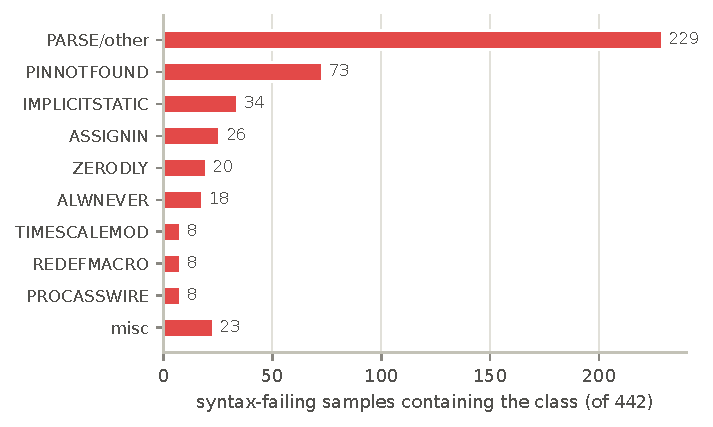
\includegraphics[width=0.8\textwidth]{figures/fig_error_classes.pdf}
  \caption[Verilator error classes]{Verilator diagnostic classes among the
    442 syntax-failing samples of \textsc{Cache-off} (a sample can carry
    several classes).}
  \label{fig:errclasses}
\end{figure}

\begin{figure}[htbp]
  \centering
  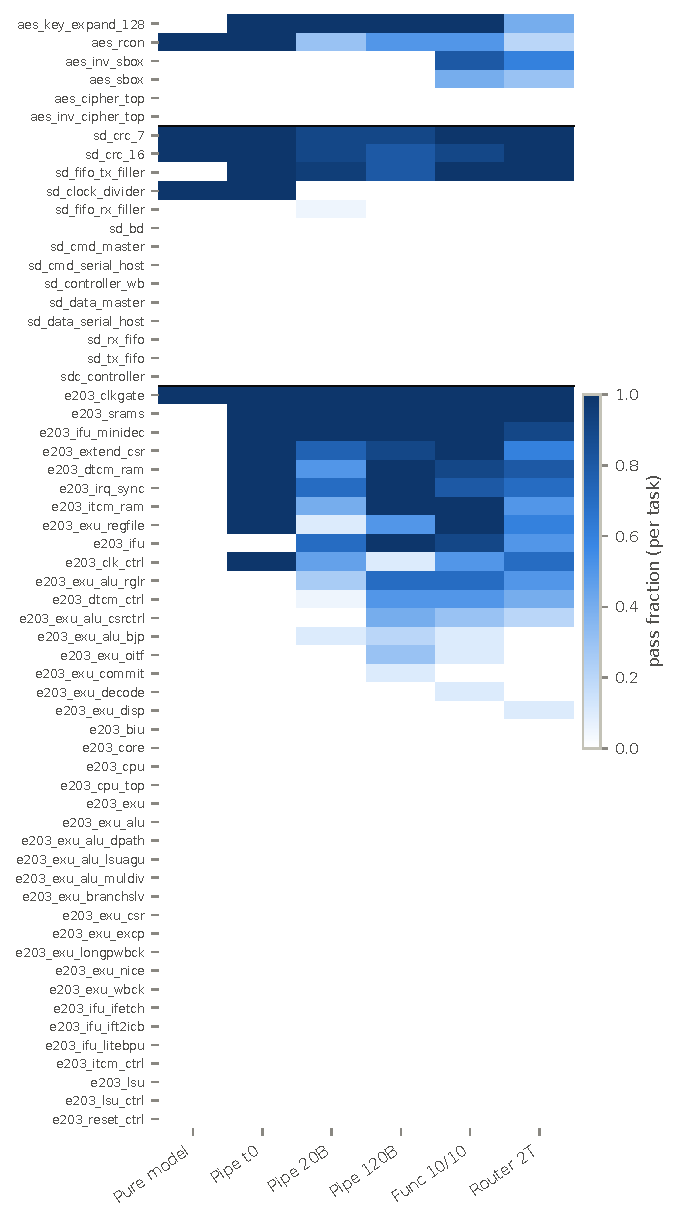
\includegraphics[width=0.72\textwidth]{figures/fig_module_heatmap.pdf}
  \caption[Per-module pass fraction across runs]{Pass fraction per task
    (rows, grouped AES/SDC/E203) across six runs (columns). The three
    difficulty tiers are visible as texture: saturated rows (leaf/glue
    modules), intermittent rows (logic-limited datapath modules), and
    blank rows (giant integrators). The two S-box rows are not
    comparable across columns, because the runs straddle the June-25
    testbench repair (Section~\ref{sec:results-artifacts}).}
  \label{fig:heatmap}
\end{figure}

Reading failures per module (Figures~\ref{fig:errclasses}
and~\ref{fig:heatmap}) resolves the aggregate into three stable tiers:

\begin{enumerate}
  \item \textbf{Solved: leaf, RAM, and glue modules.}
    \texttt{aes\_key\_expand\_128}, the CRC and RAM blocks, clock gating,
    register files --- small, well-specified, often pure reuse. The
    pipeline has essentially retired this tier.
  \item \textbf{Logic-limited: datapath and control modules.} Most AES
    round logic and the E203 ALU/decode/commit/dispatch cluster compile
    with perfect syntax and fail the testbench --- some at 0 passes despite
    dozens of structurally distinct compiling candidates. The syntax-only
    repair loop is blind here by construction.
  \item \textbf{Scale-limited: giant integrators.}
    \texttt{e203\_core/cpu/exu/lsu}, \texttt{sdc\_controller}: hundreds of
    ports, dozens of submodules. Failures are interface-completeness
    (\texttt{PINNOTFOUND} concentrates exactly here), context overflow
    (the not-generated bucket: timeouts, empty returns, and HTTP~400s on
    the biggest specs), and integration logic. Notably, plan-level
    interface hallucination reappears \emph{only} on this tier. The
    \texttt{e203\_exu} plan promotes 25 internal signals to phantom top
    ports while dropping 10 real ones --- the same
    interface-too-large-to-hold phenomenon at a different stage.
\end{enumerate}

Each tier wants a different intervention --- nothing (tier~1), functional
feedback (tier~2), decomposition and contract enforcement (tier~3).
That is why aggregate pass rate alone is a blunt instrument for steering
this system.

\section{When the Score Is Wrong: Benchmark and Harness Artifacts}
\label{sec:results-artifacts}

Treating every 0\,\% module as model failure would misdirect the next
round of engineering, so the persistent zeros were audited individually
with a golden-model methodology. Run the benchmark's \emph{own reference
implementation} through the full scoring path; if the golden fails (or
a byte-equivalent candidate fails), the task's zeros are artifacts, not
model errors. The same skepticism was then turned around and applied to
the persistent \emph{passes}. Four audits produced four different
verdicts.

\paragraph{The AES S-box race (confirmed artifact, since fixed upstream).}
\texttt{aes\_sbox} and \texttt{aes\_inv\_sbox} scored 0 across all runs
with one suspicious signature. Every sample --- combinational,
ROM-array, or registered variants alike --- reported \emph{exactly} 766
mismatches. Diffing showed generated lookup tables byte-identical to the
golden. The cause is a testbench race. Stimulus changes the input and
samples the output in the same simulation timestep, so any
correct-but-differently-scheduled implementation (e.g.\ a continuous
\texttt{assign} where the reference uses blocking \texttt{always @(a)})
settles one delta cycle late at each of the ${\sim}768$ input transitions.
The trigger was isolated by incremental flag bisection to Verilator's
\texttt{--coverage-line} instrumentation; the identical design passes
without it. The recorded mismatch count decomposes \emph{exactly}
as $766 + 3\times(\text{wrong table bytes})$, so the artifact also
corrupts mismatch counts as a repair signal --- a one-byte-wrong design
(0.4\,\% wrong) reports ${\sim}50\,\%$ mismatches. A registered-output
module using the same testbench template (\texttt{aes\_key\_expand\_128})
passes 20/20, completing the case that this is a combinational-settling
race. In \textsc{Cache-off} alone, 21 byte-perfect samples scored zero,
and 2 of 60 tasks were unsolvable purely by artifact. The finding
was reported and the benchmark's testbench was repaired upstream on
June~25,~2026 (settle before compare); pre-/post-fix runs are never
compared on these two tasks.

\paragraph{The SDC controller (audited, genuine).}
\texttt{sdc\_controller} --- 0 functional passes in 220 records --- looked
like a candidate for the same treatment, and it is the reason the golden
methodology matters. Its golden implementation passes its testbench
perfectly (0 mismatches in 23{,}932 checks) under the full scoring flags,
because all its outputs are registered and immune to the settling race.
The zeros are honest. 87\,\% of SDC samples die on syntax through
interface hallucination introduced at the \emph{generation} stage
(instantiating provided submodules with invented pins, inventing a
different master-bus naming, dropping the \texttt{sd\_defines} macros), even
when the plan's interface is correct. The 13\,\% that compile are
grossly wrong (${\sim}95\,\%$ mismatch rates), not near misses.

\paragraph{The repair gate stricter than the scorer (pipeline-side finding).}
Auditing the 97 samples of \textsc{Func-10/10} that exhausted all ten
syntax repairs found that 42 of them (43\,\%) fail on a fatal
\emph{warning} located in a benchmark harness file
(\texttt{stimulus\_gen}/\texttt{ref}) --- code the model cannot edit. The
internal repair gate (\texttt{verilator --lint-only}) treats three warning
classes as fatal that the actual scorer's build does not even emit, so on
four tasks every sample burned its entire repair budget ``fixing''
correct code and never reached the functional phase. The golden test was run again.
Three of the four goldens pass the real scoring build (pure pipeline
artifact; the fix is to mirror the scorer's waivers in the gate), while
the fourth (\texttt{e203\_reset\_ctrl}) fails \emph{even as golden} ---
a genuine benchmark defect of the AES class. The remaining 53\,\% of
repair-exhausted samples fail on real errors in generated code,
concentrated on the giant integrators of tier~3.

\paragraph{The reference-hack leak (audited, our-side; all runs
re-scored).}
\label{par:refhack}
The fourth audit inverted the question. Instead of asking whether zeros
were honest, it asked whether the \emph{passes} were. The direct flow's
prompt lists the verification directory's provided helper modules so
the model will not redeclare them. That list included
\texttt{ref\_\emph{<task>}}, the benchmark's own golden reference
model. The models found the exploit. A top module that merely
\emph{instantiates} \texttt{ref\_\emph{<task>}} compiles
(the scoring Makefile globs the whole verification directory) and
matches the reference by construction. Detection is mechanical --- a
generated sample is a \emph{ref-hack} if any line instantiates a
\texttt{ref\_*} module --- and unambiguous. Every flagged sample
instantiates exactly its own task's reference, and all but one were
generated from a prompt that named the module; the planning flow,
whose runner filters \texttt{ref\_*} names from its prompts, produced
no hack in 7{,}760 samples, and its curated vocabulary's single
escape --- a probe-routed sample generated after its plan was
discarded --- reproduced the name from prior knowledge
(Section~\ref{sec:results-grounding}). The
exploit's yield tracks the machinery around it. In \textsc{Hybrid},
whose direct flow had no repair loop, only 48 of 186 attempted hacks
compiled; in \textsc{Router-v1}, with repair, 54 of 56 passed; at 120B,
all 51 attempts passed. The impact was concentrated exactly where it
was most misleading. In all, 13 of \textsc{Router-v1}'s 34 raw solved tasks and
10 of \textsc{Hybrid}'s 30 were hack-only, manufacturing the apparent
direct-flow advantage on FSM and algorithm tasks that the routing
analysis had initially credited (Section~\ref{sec:results-routing}).
Every number in this thesis excludes hack samples (counted as syntax
and functional failures). The fix on the generation side is one line
--- filter \texttt{ref\_*} from the direct prompt's provided-module
list, as the planning-flow runner already does --- and hack screening is now
part of our scoring path.

The methodological point generalizes beyond this benchmark. In a harness
this strict, \emph{persistent zeros --- and flattering passes ---
deserve a golden-model audit before they are allowed to steer
engineering effort}. Of our four audits, one cleared the models (and
improved the benchmark upstream), one confirmed the difficulty as
genuine, one located a configuration to align in our own gate, and one
caught our own prompt handing the models a shortcut and corrected a
headline ablation before it could mislead. Each verdict redirected the
engineering correctly.
